\documentclass[10pt,twocolumn,letterpaper]{article}
\usepackage[T1]{fontenc}
\usepackage[utf8]{inputenc}
\usepackage{newtxtext,newtxmath}
\usepackage[margin=0.75in,top=0.7in,bottom=0.72in,columnsep=0.25in]{geometry}
\usepackage{microtype,graphicx,booktabs,tabularx,amsmath,xcolor}
\usepackage[numbers,sort&compress]{natbib}
\usepackage{enumitem,caption,fancyhdr,titlesec,balance,needspace}
\usepackage[colorlinks=true,linkcolor=black,citecolor=teal,urlcolor=teal,breaklinks=true]{hyperref}
\hypersetup{pdftitle={QEC-Drift: Diagnosing Noise Is Not Repairing a Decoder},pdfauthor={Logan Mann}}
\definecolor{teal}{HTML}{087E8B}
\setlength{\parindent}{1em}
\setlength{\parskip}{0pt}
\setlength{\textfloatsep}{9pt plus 2pt minus 2pt}
\setlength{\floatsep}{8pt plus 2pt minus 2pt}
\captionsetup{font=small,labelfont=bf,skip=4pt}
\titleformat{\section}{\large\bfseries}{\thesection}{0.6em}{}
\titleformat{\subsection}{\normalsize\bfseries}{\thesubsection}{0.5em}{}
\titlespacing*{\section}{0pt}{8pt plus 2pt minus 1pt}{4pt}
\titlespacing*{\subsection}{0pt}{6pt plus 1pt minus 1pt}{3pt}
\pagestyle{fancy}\fancyhf{}
\fancyfoot[L]{\scriptsize QEC-Drift \textbar{} Research manuscript \textbar{} 11 November 2026}
\fancyfoot[R]{\scriptsize\thepage}
\renewcommand{\headrulewidth}{0pt}\renewcommand{\footrulewidth}{0pt}
\setlength{\headheight}{12pt}
\setlist[itemize]{leftmargin=*,nosep,topsep=2pt}
\newcommand{\code}[1]{\texttt{#1}}
\newcommand{\D}{\mathcal{D}}
\providecommand{\doi}[1]{\href{https://doi.org/#1}{doi: \nolinkurl{#1}}}
\begin{document}
\twocolumn[{
\begin{center}
{\LARGE\bfseries QEC-Drift: Diagnosing Noise Is Not Repairing a Decoder\par}
\vspace{7pt}
{\large Logan Mann\par}
\vspace{6pt}
\end{center}
\begin{minipage}{0.98\textwidth}
\small
\textbf{Abstract.}
Scientific coding agents must turn an explanation of a changing physical system into an executable intervention. We study this gap in simulated surface-code quantum error correction. An agent receives a nominal circuit, labeled calibration shots, and an ordered, unlabeled deployment batch; it must diagnose the noise change and submit a decoder tested on hidden shots. We audit all 760 score-selected decoder episodes with exact-input transcript judgments, while retaining cohort-specific contracts and measured scores. In the selected development cohort, 144/533 episodes pass jointly. Among 321 scored episodes with a correct diagnosis, 177 fail the repair criterion. Moving-qubit faults yield 101/184 correct diagnoses but only 16/184 joint passes. A priority-ordered failure taxonomy separates harmful repairs, unchanged models, insufficient adaptation, and execution failures. Trajectory inspection identifies validation broadcasting, incorrect regime dispatch, and localization over-reporting as concrete failure paths. A frozen visible-only baseline passes 27/92 fresh within-family candidates, with wide hierarchical uncertainty; sparse model coverage precludes ranking. We release aggregate evidence and reproducible figures. These results characterize an audited development corpus, not held-out frontier-model capability or hardware performance.
\end{minipage}
\vspace{10pt}
}]

\section{Introduction}
An agent can correctly explain that a quantum processor's noise has changed and still ship a decoder that loses logical information. This distinction matters because minimum-weight matching depends on a noise model, and drift can make its weights stale. Adaptive estimation already addresses this physical problem~\citep{spitz,dgr}; neural decoders and reinforcement learning extend the space of effective interventions~\citep{alpha,alpha2,rl}. The question here is different: can a general coding agent recognize the mismatch, implement a repair, and preserve the evidence needed to explain failure?

\textbf{QEC-Drift} couples these obligations in a simulator-grounded task. Its outputs are a structured diagnosis and an executable decoder, scored separately and jointly. This makes a fluent explanation insufficient for success and exposes repairs that improve one decoding criterion while missing another. The simulator supplies planted fault structure and hidden logical observables; transcript review supplies an additional, explicitly fallible description of how an attempt unfolded.

Our contribution is an \emph{operational evaluation contract and evidence audit}, not a new decoding algorithm or a claim to the first use of agents in QEC. We (i) specify joint diagnosis and recovery criteria with oracle and custom-reference distinctions; (ii) inventory and review all 760 recorded decoder episodes without pooling incompatible cohorts into a leaderboard; and (iii) connect measured failure leaves to trace-grounded implementation defects and a frozen fresh-seed baseline. The strongest finding is a diagnosis-to-repair gap on the selected development set. The analysis also shows why high rule--judge agreement cannot substitute for validating the evaluator.

\section{Task and measurement contract}
\subsection{Visible evidence and hidden scoring}
Tasks simulate rotated surface-code memory circuits with Stim~\citep{stim} at distances 5, 7, and 9. PyMatching supplies plain and correlated matching~\citep{sparse}. The agent receives a nominal Stim circuit, labeled training and validation shots from pre-change calibration, and a chronologically ordered deployment batch containing detector events but no logical labels. Planted departures include readout changes, local qubit and gate faults, telegraph switching, spatial patches, wandering faults, and compounds. These are synthetic Pauli-noise constructions, not measurements of a physical chip or complete models of leakage and coherent noise.

The agent writes \code{decoder.py}, implementing detector-to-logical-flip prediction, and a report with adequacy, scope, stationarity, changed qubits, mechanism, confidence, and evidence. Hidden evaluation uses 300,000 shots under the task's noise process. Diagnosis $D$ checks scope and stationarity and, for local or moving faults, changed-qubit Jaccard overlap $\geq 0.5$. A local report marked nonstationary can satisfy a moving fault. Mechanism accuracy is recorded separately and is \emph{not} required for the headline pass.

\subsection{Recovery and task eligibility}
Let $L_a$ be the submitted decoder's logical error rate; $L_n$ nominal plain matching; $L_o$ correlated matching with the true noise and, when needed, the true shotwise regime; and $L_s$ the stale pre-change correlated decoder. For defined, positive reference gaps,
\begin{equation}
G=\frac{L_n-L_a}{L_n-L_o},\qquad
R=\frac{L_s-L_a}{L_s-L_o}.
\label{eq:gaps}
\end{equation}
$G$ measures nominal-gap closure; $R$ isolates drift recovery. The oracle $L_o$ has privileged simulator knowledge and is not an optimal-decoding lower bound. Thus a recovery above one is possible. Let $H=(L_s-L_h)/(L_s-L_o)$ for the stored reference $L_h$. The absolute rule requires $D$, $G\geq0.5$, and, on drift tasks, $R\geq0.5$. The reported relative rule additionally requires $R\geq0.75H$. Non-drift tasks omit the drift conditions; legacy cohorts retain the requirements actually present in their original contracts.

Drift-task admission requires the oracle to improve on the stale decoder by at least 20\% and a designated reference to recover at least half the drift loss. The stationary reference is a detector-pair correlation refit. The nonstationary reference is a \emph{benchmark-specific offline hypothesis search}: it uses the pre-drift circuit, a simulation seed, and detector time series, with a bank tailored to the fault grammar. It is neither a DGR reproduction nor an information-matched general-purpose competitor. These gates demonstrate reference decoding headroom, not that every diagnostic attribute is identifiable from every visible batch. Adequate controls are retained separately.

\section{Corpus, execution, and provenance}
\begin{table}[t]
\centering\small
\caption{Audit coverage. Every row has a current exact-input transcript judgment. Cohort contracts differ.}
\label{tab:coverage}
\begin{tabular}{lrrr}\toprule
Population & Recorded & Included & Excluded\\\midrule
Current development & 533 & 533 & 0\\
Earlier decoder cohorts & 171 & 124 & 47\\
Fresh model episodes & 56 & 56 & 0\\\midrule
All decoder episodes & 760 & 713 & 47\\\bottomrule
\end{tabular}
\end{table}
The current development corpus contains 24 model/effort configurations: 23 Codex configurations with 23 tasks each and one Claude Code configuration with four tasks. Logged model labels are GPT-5.6-Luna, GPT-5.6-Sol, GPT-5.6-Terra, GPT-6-Astra, and Opus 5.5. Provider backend weight revisions were not pinned. The 23-task core expanded after interim model results; its scores describe an adaptively selected development set. Repeated configurations share tasks, so episodes are not independent draws for a binomial confidence interval. Scaffold and effort differences also prevent interpreting this audit as a controlled comparison of model identity.

The nominal tool budget is 40 calls. The CLI runner stops at the first started call beyond that limit; archived completed-call counts range from 5 to 41. The subscription scaffolds retain network access for their provider connections and installations, while the API harness blocks network access. The former use an outer filesystem sandbox. Hidden scoring executes a throwaway copy, rather than following agent-created links. These controls reduce exposure but do not establish perfect isolation or equivalent scaffolds.

We select the archived attempt linked to each stored score. All 704 historical decoder-source records match their score rows; 541 report objects also match, with 163 lacking an archived report object. However, these historical rows have no attempt IDs, so identical-output reruns remain ambiguous. Two damaged gzip archives provide 27 recovered complete records whose checksums cannot be verified. Fresh score and event hashes are verified, but failed fresh decoder \emph{subtypes} use a later source snapshot and remain provisional. The separate 64-episode numerical-answer pilot has a different output contract and is excluded from this decoder audit.

\begin{figure*}[t]
\centering
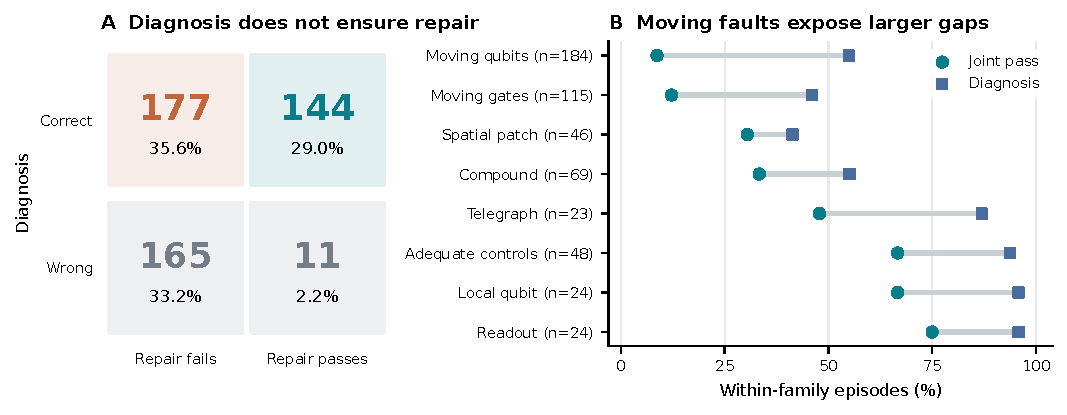
\includegraphics[width=\textwidth]{figures/diagnosis-repair.pdf}
\caption{\textbf{Diagnosis and repair are separate bottlenecks.} A: joint outcomes among the 497 development episodes with scored decoders; 36 without a score remain failures in the 533-episode headline. One unscored episode has a correct diagnosis, giving 322/533 correct diagnoses overall. B: both rates use each family's recorded denominator, including unscored episodes. Task families and configurations are dependent; these are descriptive rates. An independent recomputation from score Parquet files matches the frozen inventory: 533 episodes and 144 joint passes, discrepancy zero.}
\label{fig:outcomes}
\end{figure*}

\section{An operational failure taxonomy}
The first applicable gate in Table~\ref{tab:taxonomy} assigns one leaf. Diagnosis failure is therefore a leaf only when repair succeeds; a poor repair can also have a wrong diagnosis. This ordering produces exhaustive bookkeeping, not a complete causal theory of failure.

\begin{table}[t]
\centering\footnotesize
\caption{Priority-ordered taxonomy and development counts. G0 has 47 earlier-cohort exclusions, all absent from the development denominator. Zero-count leaves are retained.}
\label{tab:taxonomy}
\setlength{\tabcolsep}{3pt}
\begin{tabularx}{\columnwidth}{@{}clXr@{}}\toprule
Gate & Leaf & First applicable condition & $n$\\\midrule
G0 & Excluded & External invalidation & 0\\
G1 & Passed & Diagnosis and repair pass & 144\\
G2 & Budget & Deadline/budget; no score & 36\\
G3 & Missing & Stopped without a decoder & 0\\
G4 & Broken & Present but fails scoring & 0\\
G5 & Harmful & $G<0$ & 72\\
G6 & Diagnosis & Good repair; wrong diagnosis & 11\\
G7 & Nominal & Behaviorally unchanged & 44\\
G8 & Plain fitted & Fitted; lacks correlation handling & 117\\
G9 & Under-adapted & Remaining insufficient repair & 109\\\bottomrule
\end{tabularx}
\end{table}
Nominal behavior uses at least 99.99\% prediction agreement with nominal plain or correlated matching when recorded. Remaining implementation distinctions use source features, including explicit correlation-enabling calls; older rows fall back to source inspection. Such heuristics can miss custom implementations, so G7--G9 are operational evidence categories, not verified algorithm identities. The measured diagnosis and recovery requirements remain authoritative.

\subsection{Where the recorded agents fail}
Development joint success is 144/533 (27.0\%), against 322/533 (60.4\%) correct diagnoses. Of 321 scored episodes with a correct diagnosis, 177 (55.1\%) fail repair; another 11 repair successfully but fail diagnosis. The 36 unscored episodes are retained as failures. Plain fitted matching and under-adaptation account for 226/533 episodes; 72 submitted decoders are worse than nominal plain matching.

The gap is largest for moving faults (Figure~\ref{fig:outcomes}). Moving-qubit tasks have 101/184 correct diagnoses (54.9\%) but 16/184 joint passes (8.7\%). Moving-gate tasks have 53/115 diagnoses (46.1\%) and 14/115 passes (12.2\%). These comparisons mix physical settings and repeated configurations. They show where the selected corpus is difficult, not an isolated causal effect of motion or evidence that all unseen drift is difficult.

\subsection{What trajectory inspection adds}
Every score-selected decoder episode has a judgment produced by GPT-6-Astra at medium effort through the subscription CLI. Exact keys bind the input, rubric, schema, protocol, and judge settings. Known model identifiers are partially masked and the rule leaf is withheld; score facts, scaffold syntax, and tool traces remain visible. The review is model-assisted and score-aware, not independent expert ground truth. Rendering can shorten long messages and outputs; run coverage does not imply access to hidden reasoning or exhaustive review of every raw byte.

Figure~\ref{fig:trajectories} connects outcome counts to three inspected development cases. In one, comparing predictions of shape $(N,1)$ with labels of shape $(N,)$ broadcast the validation comparison to $(N,N)$; the agent subsequently chose a harmful ensemble. Another used classifier argmax indices as physical qubit IDs, breaking the routing from inferred regime to decoder. A third reported all 49 circuit qubits when 21 changed: its repair passed, but localization failed. These are concrete, purposively selected paths; we did not estimate their prevalence or intervene to identify causal effects. Tool use overlaps across leaves, so more calls alone are not a diagnosis of failure.

\begin{figure*}[t]
\centering
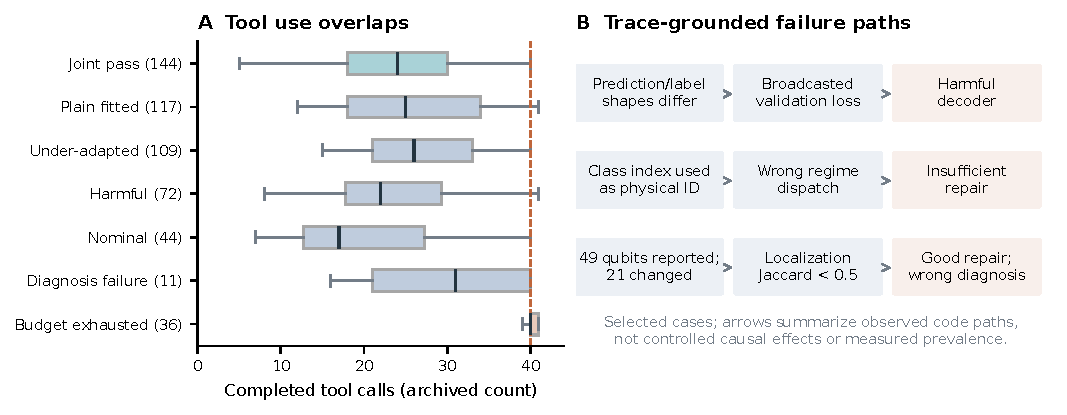
\includegraphics[width=\textwidth]{figures/trajectory-audit.pdf}
\caption{\textbf{Execution traces distinguish resource use from implementation defects.} A: completed-call distributions for all 533 development episodes; boxes show median and interquartile range, whiskers extend to 1.5 IQR, and outliers are omitted visually but retained in the data. Parentheses give sample sizes. The dashed line marks the nominal 40-call budget, not a guaranteed maximum. B: schematic reconstructions of three inspected traces. The shapes, dispatch semantics, and localization counts are observed evidence; arrows are explanations to test, not intervention-proven causes.}
\label{fig:trajectories}
\end{figure*}

\subsection{Auditing the transcript evaluator}
Rule and judge leaves agree on 700/760 episodes (92.1\%), and on 526/533 development episodes (98.7\%). These are agreement rates, not judge accuracies. Forty-seven historical traces contain a required-module import error and remain excluded by the original eligibility policy, even when an agent later recovered. The judge gives all 47 non-excluded labels. We retain both views rather than relabeling the corpus after inspection.

Four development judge labels imply sufficient repair despite a measured recovery below 0.5: two false pass assignments and two diagnosis-failure assignments. Raw judgments and stored scores are preserved. This deterministic consistency check detects a specific contradiction and does not estimate the judge's full error rate. Automated integrity concerns appear in 289/533 development reviews, including installs and boundary probes; these flags do not prove cheating, access to test labels, or a causal reason for failure. High agreement and a favorable fairness judgment are insufficient certification of an evaluator~\citep{judge,quantumaudit}.

\section{Frozen fresh-seed replication}
A fixed visible-only baseline provides a separate within-family check. It compares deployment detector rates with 20,000 nominal simulated shots, using 99 whole-shot permutations and a $p\leq0.01$ adequacy threshold. A multiscale block statistic tests shot order with a second permutation test. Localization unions the custom adaptive bank's hypotheses supported by at least 50 deployment shots. The decoder uses nominal correlated matching, a deployment refit, or the adaptive bank according to the inferred scope. This is a custom, development-informed baseline, not a new general decoder or a reproduction of DGR.

Before fresh evaluation, its implementation, candidate manifest, seeds, gates, resource limits, and predictions were frozen. The study changes locations and shot seeds within 23 selected templates from nine families. Of 92 candidates, 85 meet the frozen eligibility gate. The baseline passes 27/92 overall (29.3\%) and 26/85 eligible cases (30.6\%). A 10,000-draw hierarchical bootstrap over families, templates, and replicates gives descriptive 95\% intervals of 11.6--61.5\% and 11.8--67.6\%, respectively. Few clusters and no model-sampling repeats limit interpretation.

All 18 baseline scoring errors hit the fixed 300-second deadline and remain failures. Adequacy is correct on 92/92, full diagnosis on 41/92, and mechanism on 36/92. In 80 localized cases, the predicted set is larger than truth in 71, equal in six, and smaller in three. The mean prediction contains 27.875 qubits against 15.913 changed qubits. Thus detecting inadequacy is much easier for this baseline than localizing a complete fault precisely.

Fresh model execution completed only 56 valid episodes across 22 configurations: 53 scored, three score errors, and 13 relative passes (14 absolute). The planned schedule had 5,336 configuration--candidate pairs, 4,930 eligible. Execution stopped at a credential-lifetime preflight; the Claude usage probe failed, so no fresh Claude episode was admitted. Only 38 comparisons have any matched candidates and the largest covers 6/85 eligible candidates. Missing episodes are availability omissions, not model failures. These data do not support ranking configurations or comparing their pass rate with the fully evaluated visible baseline.

\section{Related work and novelty boundary}
\textbf{Adaptive QEC and learned decoding.} Syndrome-based adaptive weight estimation~\citep{spitz} and DGR's graph reweighting~\citep{dgr} already address drift and correlations. AlphaQubit~\citep{alpha}, its scalable successor~\citep{alpha2}, and experimental RL steering~\citep{rl} demonstrate learned decoding or control. We neither supersede those methods nor show improved logical performance. Our object is an agent's coupled scientific diagnosis, code artifact, and recoverable evidence under a changing simulator model.

\Needspace{3\baselineskip}
\textbf{Quantum coding agents.} QCoder~\citep{qcoder} and QuanBench+~\citep{quanbench} evaluate generated quantum programs; StabilizerBench~\citep{stabilizer} evaluates QEC circuit synthesis with simulation-based verification. The online SSI surface-code environment also asks an agent to develop a decoder from experimental data.\footnote{Verified project artifact, not a paper: \url{https://openssi.dev/ssi-index/environments/surface-code-decoding/}, accessed 11 November 2026.} Therefore agent-written decoders and simulator-grounded quantum evaluation are not novelty claims. We focus on a nominal-to-deployment shift, explicit planted-fault diagnosis, a joint recovery criterion, and an audit that preserves score/trace disagreements. Quantum SDK API drift~\citep{apidrift} concerns software-version fidelity rather than physical noise drift. Seefried et al.~\citep{quantumaudit} already show that quantum-code evaluation defects can dominate apparent performance; our source-binding and judge-consistency audit applies that concern to diagnosis-and-repair episodes.

\textbf{Scientific agents and failure analysis.} SciCode~\citep{scicode}, ScienceAgentBench~\citep{scienceagent}, MLE-bench~\citep{mle}, PaperBench~\citep{paperbench}, SciAgentGym~\citep{scigym}, and SciAgentArena~\citep{sciarena} evaluate scientific coding, tool use, engineering, or research workflows. QEC-Drift trades that breadth for simulator-derived fault truth and separate diagnosis and repair axes. MAST~\citep{mast} provides a broader trace-based taxonomy for multi-agent systems; our priority tree is a narrower operational partition of decoder outcomes. Unlike expert-validated annotation, the present model-assisted review does not establish human inter-rater reliability.

The novelty check searched primary papers and project artifacts across these neighboring areas through 11 November 2026. No global ``first'' or exhaustive-coverage claim follows from targeted retrieval. The defensible contribution is the combined evaluation contract and audited corpus. A source-by-source overlap matrix, query record, and bibliographic metadata accompany the LaTeX source.

\section{Limits, release, and next experiment}
The development set was adapted after interim results; fresh seeds remain within selected families; scaffold conditions and provider versions differ; historical attempt linkage is imperfect; subtype rules are heuristic; and the transcript judge is not independent. Raw traces may expose local paths and candidate identities, so only anonymous aggregates and checked case summaries are distributed. Public aggregates reproduce the figures, not a full independent replay of private trajectories. No hosted Kaggle run or physical-device experiment is reported. Unrun grid cells remain unrun.

The next decisive experiment is a frozen, matched evaluation on unseen fault families with repeated model samples, uniform budgets, an independently implemented reference, and blinded human review of a stratified trace sample. Candidate interventions include shape-safe validation, typed physical-ID dispatch, early fallback submission, and separately calibrated localization precision/recall. They are testable hypotheses, not measured improvements.

QEC-Drift's present result is that diagnosis and decoder repair separate sharply in this recorded corpus. Reliable scientific agents need both, and their evaluation must retain failed execution, disputed exclusions, and evaluator contradictions alongside successful runs.

\paragraph{Artifact and reproducibility.}
Code and aggregate audit: \href{https://github.com/itsloganmann/qec-drift-bench/tree/c02efe99308605ace6c47cb700382fa9d05af02a}{\texttt{github.com/itsloganmann/qec-drift-bench}}, public snapshot \code{c02efe9}. The source bundle includes anonymous plot inputs, figure-generation code, the literature audit, and build instructions. The paper introduces no additional model runs and changes no historical scores.

\clearpage
\begingroup
\small
\setlength{\bibsep}{3pt plus 1pt}
\balance
\bibliographystyle{abbrvnat}
\bibliography{references}
\endgroup
\end{document}
